\pagelayout{margin}
\setchapterstyle{kao}
\setchapterpreamble[u]{\margintoc}
\chapter{Results}
\label{ch:results}

In this chapter, we present and analyze the results of our prediction model. First, a quantitative comparison with other models is provided using various error metrics to evaluate the model's performance. Next, we analyze the latent profiles learned by our model and examine how they are utilized in predictions. We then assess the model's ability to predict total power consumption. Finally, we summarize the key findings from our experiments and their implications.

\section{Quantitative comparison with other models}
\label{sec:res-comparison}


Based on the defined loss functions in Chapter \ref{ch:research}, we present the loss of the model. The losses represent error on prediction for an hour, calculated by dividing the loss by 24, instead of using the 24 values representing a full day.

The losses can be seen in Table \ref{tab:losses-table}.

\begin{table*}[h!]
    \begin{tabular}{p{3cm} p{1.5cm} p{2cm} p{1.3cm} p{1.3cm} p{2cm} p{1.6cm} p{1.6cm}}

        \toprule

        \textbf{Model name}          & \textbf{MAE}                         & \textbf{MSE}                         & \textbf{MAE norm profile}         & \textbf{MSE normal profile}       & \textbf{MSE total power}          & \textbf{MAE total power}             & \textbf{MSE mixture loss}         \\

        \midrule

        Latent profiles NN           & $3.6717$                             & $1661.9267$                          & $0.0021$                          & $0.0003$                          & $3.5574\times10^{5}$              & $64.0718$                            & $3.4302$                          \\

        Latent profiles NN (no data) & $3.7540$                             & $1667.8263$                          & $0.0020$                          & $0.0003$                          & $3.5677\times10^{5}$              & $66.3788$                            & $3.4138$                          \\

        Train average                & $3.8964$                             & $1664.8744$                          & $0.0021$                          & $0.0003$                          & $3.5561\times10^{5}$              & $69.6754$                            & $3.4125$                          \\

        Test average model           & $3.8964$                             & $1664.8744$                          & $0.0021$                          & $0.0003$                          & $3.5561\times10^{5}$              & $69.6754$                            & $3.4125$                          \\

        Linear regression            & $4.2535$                             & $1823.4076$                          & $0.0060$                          & $0.1130$                          & $4.0771\times10^{5}$              & $79.0246$                            & $1130.0005$                       \\

        XGBoost                      & $4.0460$                             & $2430.1903$                          & $0.0022$                          & $0.0004$                          & $3.9855\times10^{5}$              & $68.6162$                            & $4.1041$                          \\

        \midrule

        \textbf{Difference \%}       & $\textcolor{ForestGreen}{+6.1204\%}$ & $\textcolor{ForestGreen}{+0.1774\%}$ & $\textcolor{BrickRed}{-1.7618\%}$ & $\textcolor{BrickRed}{-0.5702\%}$ & $\textcolor{BrickRed}{-0.0377\%}$ & $\textcolor{ForestGreen}{+8.7459\%}$ & $\textcolor{BrickRed}{-0.5150\%}$ \\

        \bottomrule
    \end{tabular}
    \caption{Table containing losses for several metrics. The last difference row provides percentage comparison between latent profiles NN model and train average.}
    \label{tab:losses-table}
\end{table*}

From inspection of the table, it can be seen that the model did not provide better results. We hypothesize that the model derived most of its performance from learning to predict the average. We conclude that the current features we used for predicting power consumption did not help the model perform better.

\section{Latent profiles analysis}

Although our model's prediction quality was not improved, the model learned to utilize the latent profiles. In this section, we examine how the model learned to utilize these profiles. To reiterate, we hypothesized that charging demand can be modeled as a mixture of $K$ charging profiles, and meaning could be derived from both the learned profiles and the prediction of probabilities per location.

\begin{figure}
    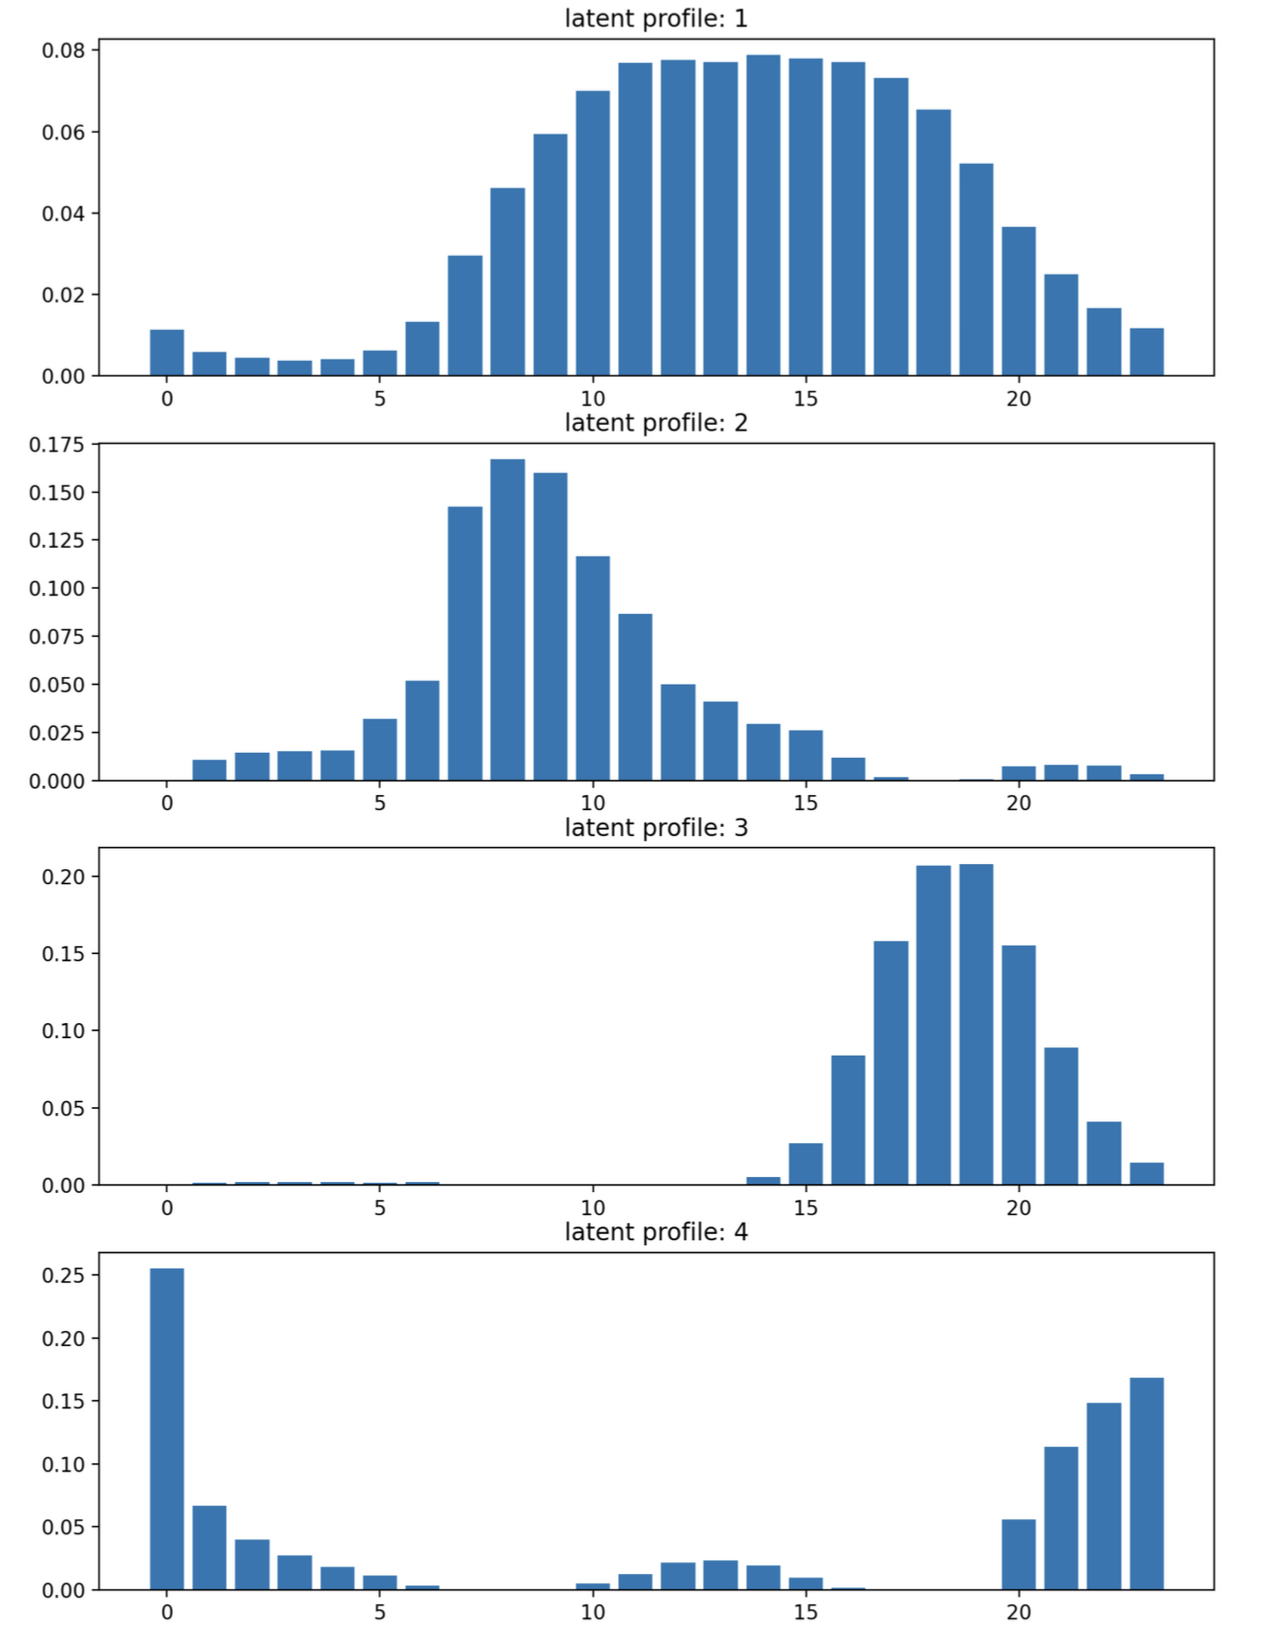
\includegraphics[width=0.7\textwidth]{learned-latent-profiles.png}
    \caption{Latent profiles learned by our model}
    \label{fig:learned-latent-profiles}
\end{figure}


\begin{marginfigure}
    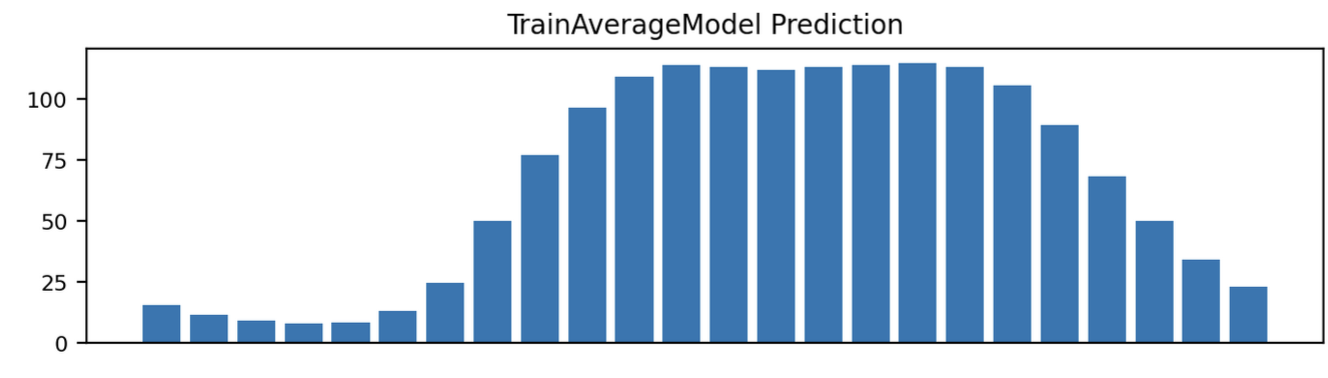
\includegraphics{train_average.png}
    \caption{Train dataset $\mathcal{T}$ labels average}
    \label{fig:train_average}
\end{marginfigure}

\begin{marginfigure}
    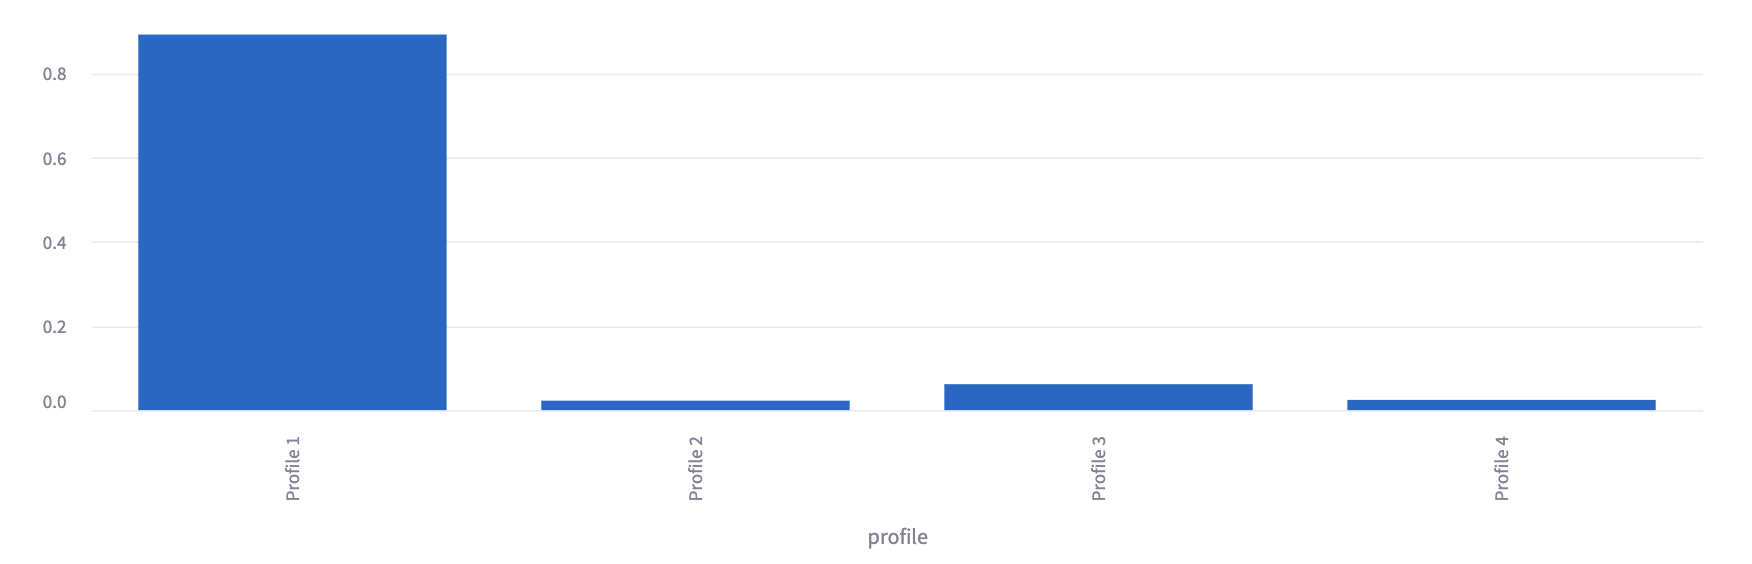
\includegraphics{average_probs.png}
    \caption{Average predicted latent profile probabilities by our model on the train dataset.}
    \label{fig:average_prob}
\end{marginfigure}

\begin{marginfigure}
    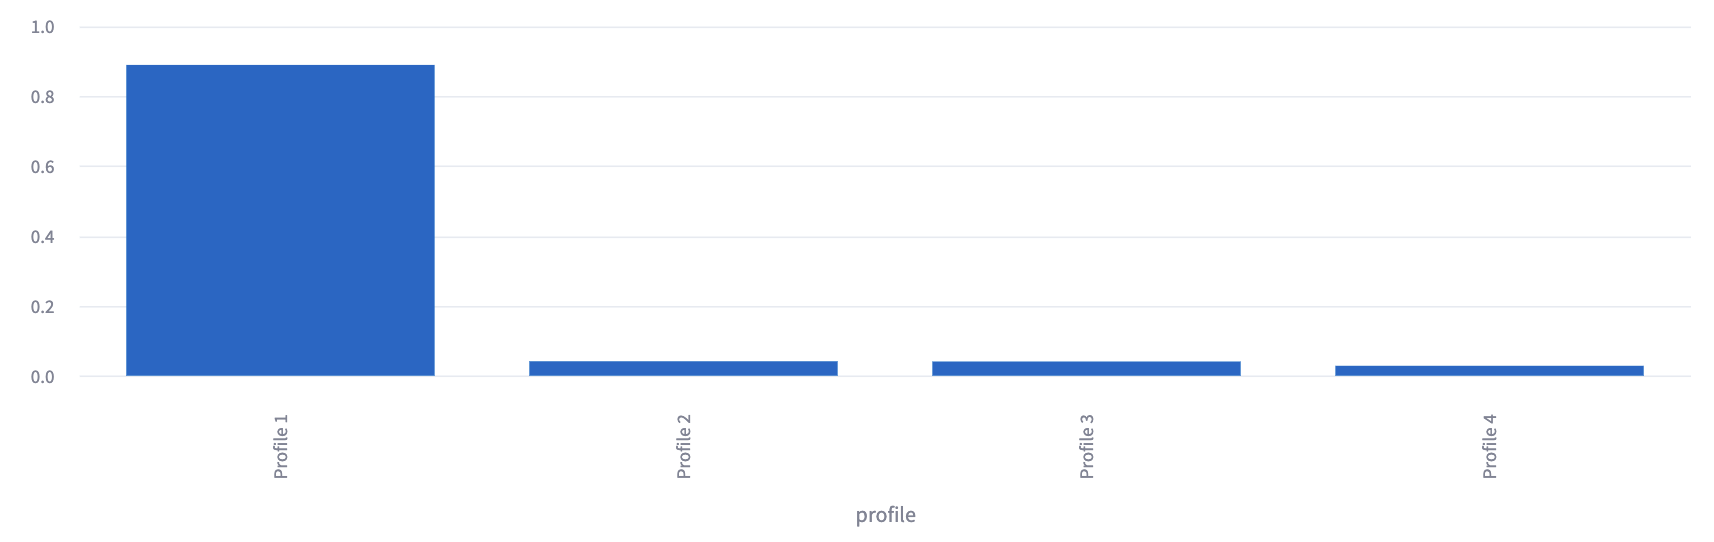
\includegraphics{average_probs_test.png}
    \caption{Average predicted latent profile probabilities by our model on the test dataset.}
    \label{fig:average_prob_test}
\end{marginfigure}

We found that setting $K=4$ was the lowest possible number at which the train and validation loss could not be improved further.

The learned profiles are visible in Figure \ref{fig:learned-latent-profiles}.

The first profile closely corresponds to the average over the train dataset $\mathcal{T}$ labels (see Figure \ref{fig:train_average}). While also resembling the average power consumption of the ZSJ unit of "compact residential area" (see Figure \ref{fig:zsj-charging-impact}). A large part of the predictions for data from the test dataset utilize this profile (see Figure \ref{fig:average_prob_test}). We interpret this as our model falling back to simply giving the average of "compact residential area" chargers as its prediction\sidenote{This could be mitigated by stratified sampling}.

\section{Power consumption}

The second part of what our model predicts is the total power, of .This was already hypothesized in the beginning section, due to the absence of data about charger maximum power output. The comparison of true values versus predicted values can be seen in Figure \ref{fig:total-power-comparison}. This may be due to the absence on the chargers

\begin{figure}[h!]
    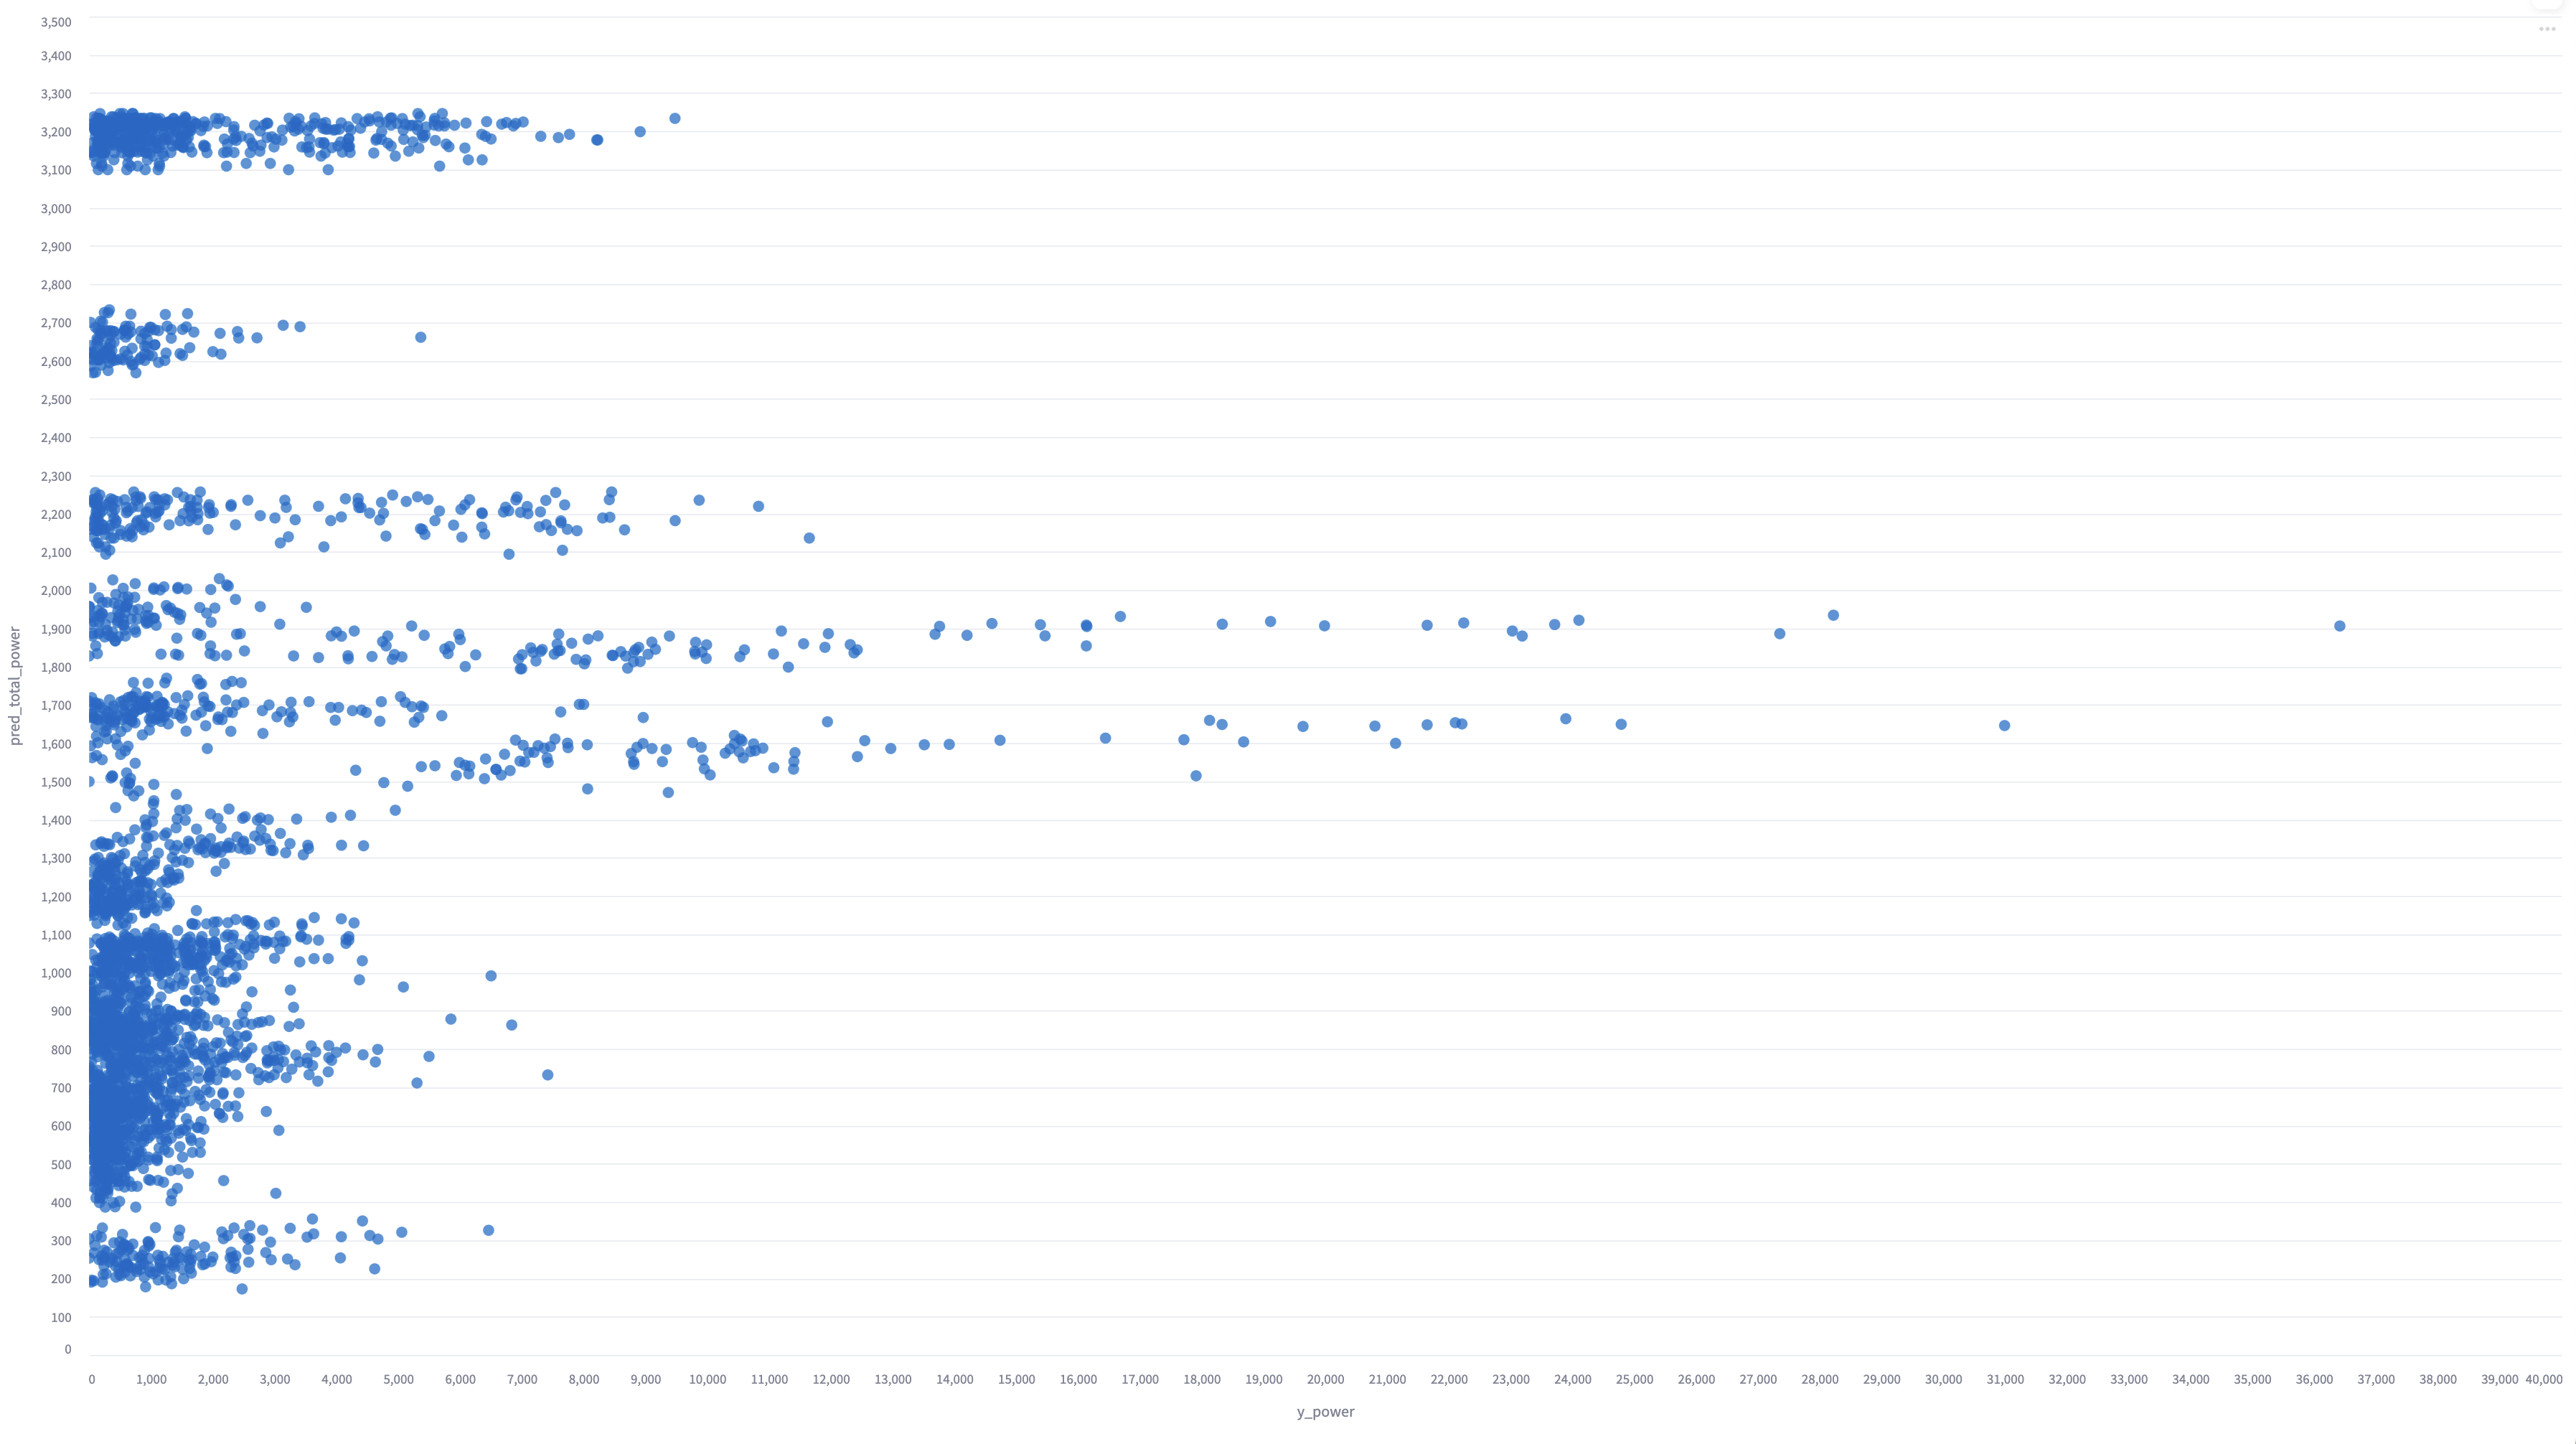
\includegraphics{total_power_comparison.png}
    \caption{Comparison of true total power (x axis) and our prediction (y axis)}
    \label{fig:total-power-comparison}
\end{figure}

\section{Conclusion}

The takeaway from our findings is that the data used for the model were not sufficient and would require gathering a larger dataset of features. Potential additional data sources will be discussed in the conclusion. This could also be attributed to the fact that the model did not manage to fit the training dataset well.
